\section{Architectural Decisions}
\label{se:architectural_decisions}

The initial design of \acrshort{wdias} used the \acrfull{soa}. Moreover, it tried to use an \acrfull{esb} to integrate different modules, as \acrshort{esb} could act as a shared layer for all of the modules to interact together. By default, \acrshort{esb} also provides publisher/subscriber capabilities.

The \acrshort{esb} processing units called \emph{mediators}. A mediator can take a message, carry out some predefined actions on it, and output the modified message. These mediator capabilities can be used to integrate the modules of a weather data system, as shown in \cref{fi:wdia_components}. \acrshort{esb} also supports different transportation protocols such as HTTP and web sockets. However, we realized that \acrshort{esb} is not suitable for data streaming or bulk data processing. Also, \acrshort{esb} suffers from a single point of failure, as all the messages are going through a common shared bus and slower communication (cannot be used for transfer data). In the second design phase of \acrshort{wdias}, we attempted to use the actor model using the AKKA framework \cite{HewittWhyModel} to overcome above \acrshort{esb} drawbacks. At the same time, we moved away from the \acrshort{soa} architecture design to the microservice architecture design.

Thus, we redesigned the system architecture with decomposing into microservices and used actors to implement each microservice in the system. In that case, we mapped each microservice in \acrshort{wdias} to an actor or an actor with slave actors. \acrshort{soa} focuses on imperative programming, while the microservices architecture focuses on a reactive actor programming style using faster messaging mechanisms.
When compared to \acrshort{soa}, the microservice architecture has several advantages:
\begin{itemize}
    \item Follow the principle of a single responsibility.
    \item Resilient/flexible because a failure of service does not influence other services. If you have monolithic or significant service errors in a service/module, this can have an impact on other modules/functionalities.
    \item High scalability because demanding services can be deployed on different servers to improve performance and stay away from other services so that they do not affect other services. It will be challenging to achieve the same with a single large monolithic service.
    \item Easy to improve the system because the microservices are decoupled from other services. It is also easier to change and test each microservices.
    \item Little impact on other services because each service is independent.
    \item Easy to understand because they represent a small functionality.
    \item Ease of deployment.
\end{itemize}

The AKKA framework has some of the disadvantages of implementing each microservice as an actor, as described in AKKA documentation \cite{Akka.ioWhenCluster}. One of the attractive features of microservice architecture is the independent nature of the microservices. The above concept allows choosing different technologies for each microservice based on the advantage that could bring in. Also, the microservice architecture will enable us to independently develop and maintain a system by multiple smaller and more focused teams/communities. But using the actors as microservice, the actors communicate using message passing cause to result in a too-tight code coupling between the services and difficulty to deploy services independent of each other, which is one of the main reasons for using a microservices architecture \cite{Akka.ioWhenCluster}. To overcome these problems, we moved to the concept of container orchestration based microservice architecture.

Containerization is an alternative to virtualization that supports virtual machines or hypervisors. It includes encapsulating or grouping the software code and all its dependencies so that it can work uniformly and consistently in any infrastructure \cite{IBMContainerizationExplained}. The concept of containerization and process isolation has emerged after the open source Docker Engine \cite{DockerAppContainerization}, an industry standard for package software into standardized units for development, shipment, and deployment.

\acrshort{wdias} used \acrfull{k8s} as the container orchestration system. \acrshort{k8s} is an open-source tool for automating deployment, scaling, and management of containerized applications [15]. It groups the containers that make up an application into logical units for easy management and detection. Using \acrshort{k8s}, we deploy each microservice as a container and manage it by providing scalability and availability.

\begin{figure}[htp]
    \centering
    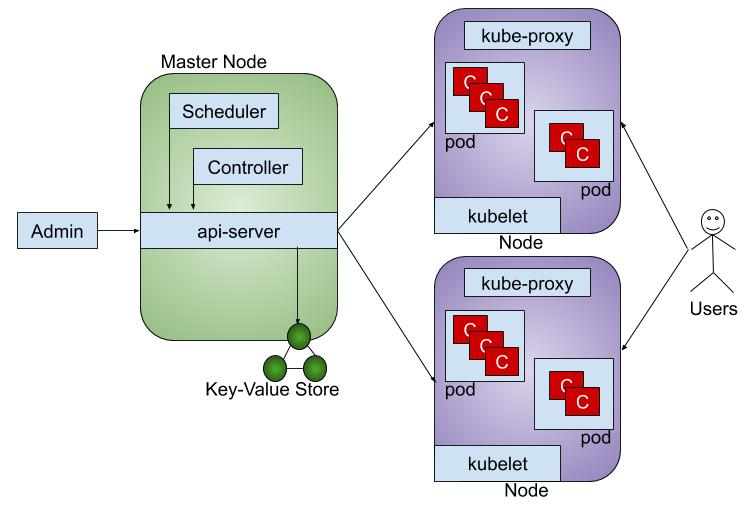
\includegraphics[width=1\textwidth]{method/microservice/k8s_architecture_v3.jpg}
    \caption{\acrfull{k8s} architecture.}
    \label{fi:k8s_architecture}
\end{figure}

\cref{fi:k8s_architecture} give an overall idea on the components of \acrshort{k8s},
\begin{itemize}
    \item Pods -- Cluster of containers that can group other container images in a single unit.
    \item Nodes -- The machines (VMs, physical servers, etc) in a cluster that runs your applications and cloud workflows.
    \item Kubelet -- An agent that runs on each node in the cluster. It makes sure that containers are running in a pod.
    \item Kube-proxy -- A network proxy that runs on each node in the cluster, and maintains network rules on nodes.
    \item Kubernetes master -- Responsible for maintaining the desired state for your cluster.
    \item etcd -- Consistent and highly-available key value store used as \acrshort{k8s} backing store for all cluster data.
\end{itemize}

Users can add nodes much as required into the \acrshort{k8s} cluster, and \acrshort{k8s} manage and deploy applications as pods into cluster nodes. Each microservice can deploy as a pod, which is a group of containerized applications. \acrshort{k8s} is able to scale as much as the user requirements by deploying multiple copies of the same pod. By separating each microservice as a container, and running them as multiple pods inside the \acrshort{k8s} removes the tight coupling of microservices when compared to the actors. It preserves the independent nature of the microservices and supports the high scalability of the system.

%%%%%%%%%%%%%%%%%%%%%%%%%%%%%%%%%%%%%%%%%%%%%%%%%%%%%%%%%%%%%%%%%%%%%%%%%%%%%%%%
% Architecture Comparison with Existing Systems
\begin{table}[htp]
    \caption{Comparison of features among existing weather data assimilation and integration systems and \acrshort{wdias}. }
    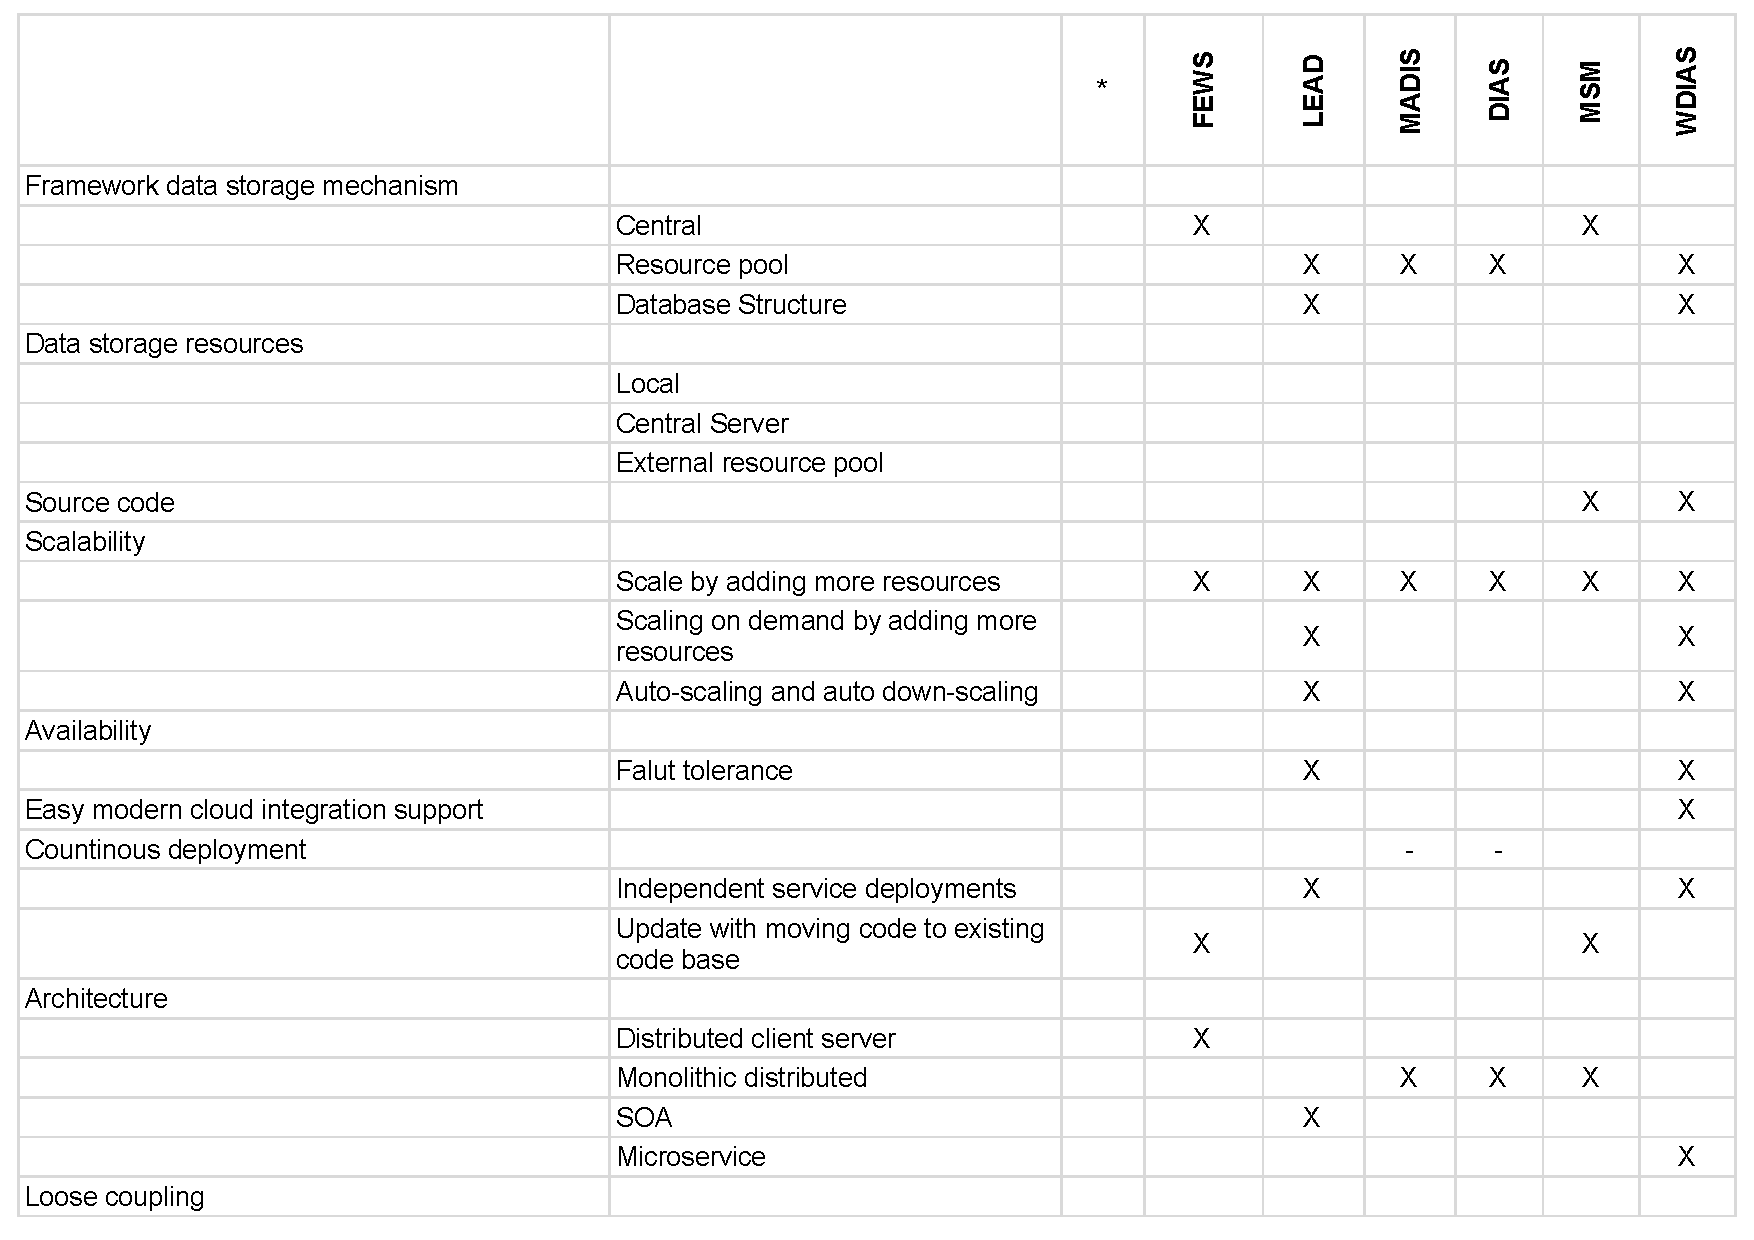
\includegraphics[width=1\textwidth]{method/misc/architecture_comparison_pros_cons.pdf}
    \label{tab:architecture_comparison}
    {\raggedright \footnotesize An "\Cross" in the table represents a feature offered by the corresponding tool. An "\SmallHBar" in the table represents that information available are not enough to make an statement, and empty presents a feature is not offered. \par}
\end{table}

\cref{tab:architecture_comparison} shows a comparison between existing systems and WDIAS concerning software architectural aspects. Here, we compare systems under categories such as data storage, performance, architecture, and other features. The \acrshort{fews} and \acrshort{msm} frameworks store the data on a central data service, which could become a bottleneck while handling large volumes of data in a critical situation. Other systems can use a pool of resources allowing them to increase the performance by adding more resources to the system. Regarding the performance of the systems, we consider scalability, availability, cloud computing support, and system deployment capabilities. All the systems can scale up to some extent by adding resources beforehand or in real-time. However, LEAD, DIAS, and WDIAS could scale on-demand by adding more resources and support automatic elasticity (i.e., scaling up and down). LEAD, MADIS, DIAS, and WDIAS have high availability, as they use a resource pool that can run on different locations. Further, these systems are capable of automatically handling partial system failures enabling fault tolerance. When we consider cloud computing support, the system should support easy integration with clouds. It is possible to rent virtual servers and deploy the local services in the cloud infrastructure, but some systems may not allow access to them remotely. Even though some systems can deploy in such a manner, they may not be capable of automatically allocating resources on demand. Hence, we cannot consider that those systems can utilize cloud infrastructures fully. Furthermore, we can easily maintain a system if it consists of independent subsystems, and each subsystem is capable of deploying or upgrading independently. Independent service deployment is a more flexible and better way to handle this, rather than copy-pasting codes to deploy changes.

We discuss the architecture of the systems in terms of their design, dependencies of the subsystems, extensibility, availability of source code, and data preprocessing capabilities specific to the weather domain. While other existing systems use distributed client-server architecture or monolithic distributed architecture \cite{ChristensenBenDontMonolith}, LEAD uses the SOA architecture. However, WDIAS has the advantage of using modern cloud computing technologies to implement microservices as containerized applications. The architecture implementation of independent subsystems allows users to maintain subsystems independently. Further, WDIAS enables different subsystems to be implemented using different technology stacks. Specially WDIAS and MSM provide an open-source framework that gives users the capability to enhance or modify the system as per the requirement. These systems provide data preprocessing capabilities for weather data and the ability to add new preprocessing capabilities. However, WDIAS is also capable of providing auto-scaling with data preprocessing. Workflow engine and model execution support are some other extra features that are helpful with weather forecasting. However, the WDIAS focuses on implementing a WDIA system with supporting main features, and it provides an extendable open framework to integrate such features easily.
